% =====================================================================
% 英语元音范畴合并的跨母语比较与发音诊断效度验证
% 全流程工作报告
% 编译：xelatex main.tex （跑两遍以生成目录与交叉引用）
% =====================================================================
\documentclass[11pt,a4paper]{ctexart}

% ---------- 页面 ----------
\usepackage[top=2.5cm,bottom=2.5cm,left=2.6cm,right=2.6cm]{geometry}
\usepackage{amsmath,amssymb,bm}
\usepackage{booktabs,longtable,array,multirow}
\usepackage{enumitem}
\usepackage[table]{xcolor}
\usepackage{graphicx}
\usepackage{caption}
\usepackage{titlesec}
\usepackage{fancyhdr}
\usepackage{lastpage}
\usepackage[colorlinks=true,linkcolor=blue!55!black,citecolor=blue!55!black,
            urlcolor=blue!55!black]{hyperref}

% ---------- 字体 ----------
\usepackage{fontspec}
\setmainfont{Times New Roman}
\setsansfont{Arial}
\setmonofont{DejaVu Sans Mono}
\usepackage{xeCJK}
\setCJKmainfont{SimSun}
\setCJKsansfont{SimHei}
\setCJKmonofont{SimSun}

% ---------- 标题样式 ----------
\titleformat{\section}{\heiti\large}{\thesection}{0.8em}{}
\titleformat{\subsection}{\heiti\normalsize}{\thesubsection}{0.7em}{}
\titleformat{\subsubsection}{\heiti\normalsize}{\thesubsubsection}{0.6em}{}
\titlespacing*{\section}{0pt}{1.6ex plus .2ex}{1.0ex}
\titlespacing*{\subsection}{0pt}{1.2ex plus .2ex}{0.8ex}

% ---------- 图与表 ----------
\graphicspath{{../figs/zh/}}
\captionsetup{font=small,labelfont=bf,labelsep=quad}
\captionsetup[table]{skip=4pt}
\renewcommand{\arraystretch}{1.15}

% ---------- 页眉页脚 ----------
\pagestyle{fancy}
\fancyhf{}
\fancyhead[L]{\small 英语元音范畴合并的跨母语比较与发音诊断效度验证}
\fancyhead[R]{\small\thepage/\pageref{LastPage}}
\renewcommand{\headrulewidth}{0.4pt}

% ---------- 常用命令 ----------
\newcommand{\ipa}[1]{/#1/}
\newcommand{\figref}[1]{图~\ref{#1}}
\newcommand{\tabref}[1]{表~\ref{#1}}

\title{\heiti\LARGE 英语元音范畴合并的跨母语比较\\[4pt]
       \heiti\LARGE 与发音诊断效度验证\\[10pt]
       \normalsize\normalfont 全流程工作报告}
\author{}
\date{\today}

\begin{document}

% =====================================================================
\begin{titlepage}
\centering
\vspace*{3.5cm}
{\heiti\LARGE 英语元音范畴合并的跨母语比较}\\[8pt]
{\heiti\LARGE 与发音诊断效度验证}\\[28pt]
{\Large 全流程工作报告}\\[60pt]
{\large
\begin{tabular}{rl}
数据规模 & 31 位说话者，7{,}750 条录音，78{,}293 个元音样本\\[3pt]
分析方法 & 音素级对齐 · 声学测量 · 混合效应模型 · 置换检验\\[3pt]
主要产出 & 跨母语证据 · 诊断工具 · 可复现流程\\
\end{tabular}}\\[80pt]
{\large \today}
\vfill
\end{titlepage}

% =====================================================================
\begin{abstract}
\noindent
本研究针对二语语音教学"反馈依赖主观听感、缺少客观诊断手段"的问题，构建了一套可解释的
英语元音发音诊断方法，并对其效度进行了实验验证。

研究采用对照设计：31 位说话者朗读\textbf{完全相同的 250 个句子}，其中 24 位为六种母语背景的
二语学习者（含 5 位普通话母语者），7 位为英语母语者，共获得 7{,}750 条录音与 78{,}293 个
元音样本。经音素级对齐后提取元音中点共振峰、元音时长与语速，在 Bark 标度上做说话人内
Lobanov 归一化，以混合效应模型、置换检验与效应量进行统计推断。

主要结果有三。其一，学习者的困难并非元音空间整体缩小：面积差异仅为趋势
（$p=0.095$），但局部的 \ipa{ɑː}–\ipa{ʌ} 距离仅为母语者的 42\%（$d=-3.83$），
\ipa{ɪ}–\ipa{iː} 为 34\%（$d=-2.43$）。其二，\textbf{跨六种母语背景的比较表明，这种
范畴合并不是普通话特有的母语迁移}：七组整体差异显著（$p=0.002$），但普通话与其他二语组
无差异（$p=0.73$），西班牙语与越南语的合并程度更强。其三，学习者的元音时长对比与语速
亦系统性偏离（时长比 1.13 vs 1.27，趋势；语速 2.89 vs 3.64 音节/秒，$d=-2.51$）。

研究进一步以母语者参照分布构建马氏距离评分，并与自动语音识别词错率对照：学习者 24.0\%
vs 母语者 7.7\%，评分与可懂度的 Spearman $\rho=0.937$（母语者组内 $\rho=1.000$）。据此
实现的诊断工具可输出逐元音的偏离度、时长诊断与教学建议。

\vspace{6pt}
\noindent\textbf{关键词：}二语语音；元音空间；范畴合并；母语迁移；发音诊断；可懂度
\end{abstract}

\newpage
\tableofcontents
\newpage

% =====================================================================
\section{引言}

\subsection{研究背景}

中国英语学习者的发音问题长期存在，但课堂反馈高度依赖教师的主观听感：同一位学生的同一段
朗读，不同教师可能给出不同判断，且难以说明"错在哪、该怎么改"。这种定性反馈难以规模化，
也难以追踪进步。

从语音学角度看，发音的可测量部分是声学参数。元音的音质主要由前两个共振峰（F1、F2）决定，
二者分别对应舌位高低与前后；元音之间的声学距离因而可以直接反映"两个音是否被区分开"。
这一可测量性，使得"把主观判断转化为客观诊断"在技术上成为可能。

\subsection{研究问题}

本研究围绕三个问题展开：

\begin{enumerate}[leftmargin=2em,itemsep=2pt]
  \item 二语学习者的元音系统与母语者相比，差异是\textbf{整体性}的（空间收缩）还是
        \textbf{局部性}的（特定范畴合并）？
  \item 若为局部合并，它是否由母语背景决定？即，是否可以用"母语迁移"解释？
  \item 基于声学偏离构建的诊断评分，是否真的对应"别人能不能听懂"？
\end{enumerate}

\subsection{主要贡献}

\begin{enumerate}[leftmargin=2em,itemsep=2pt]
  \item \textbf{跨母语证据}：在六种母语背景、31 位说话者上，用统一对照设计检验了
        \ipa{ɪ}–\ipa{iː} 范畴合并，发现其为二语学习的普遍困难而非某母语特有，
        修正了流行的"母语迁移"解释。
  \item \textbf{方法对比}：证明整体性指标（元音空间面积）会掩盖局部效应，
        而元音对距离能揭示 $d<-3$ 量级的差异。
  \item \textbf{效度验证}：把诊断评分与自动语音识别词错率逐人对照
        （$\rho=0.937$），为"评分确实反映可懂度"提供了外部证据。
  \item \textbf{可复现实现}：从原始音频到诊断输出，全流程脚本化，并配以发表级图件。
\end{enumerate}

% =====================================================================
\section{相关工作}

\subsection{二语元音的声学研究}

二语元音的声学对比已有大量积累。近年一项发表于 \textit{JASA} 的研究系统比较了普通话母语者
与英语母语者对英语松紧元音的产出，发现学习者在静态与动态频谱特征上均存在系统性差异
\cite{jasa2024}。这类研究确立了"用共振峰测量二语元音"的范式，但多数只涉及单一母语背景。

\subsection{元音空间与可懂度}

元音空间面积（vowel space area, VSA）是衡量发音"清晰度"的经典指标。已有研究表明，
元音空间较大的说话者通常更易被听懂 \cite{bradlow1996}。但 VSA 对个体差异极为敏感，
在样本量有限时检验功效不足，这一点在二语研究中常被忽略。

自动语音识别（ASR）作为可懂度的客观代理已被验证：有研究比较了 ASR 与母语听辨者对二语
语音的评分，发现两者的错误类型与比例高度相似 \cite{recall}。这为"用 ASR 词错率作为
可懂度代理"提供了依据。

\subsection{发音诊断工具}

面向学习者的元音工具已有若干。\textit{Visible Vowels} 是一个成熟的网页应用，可对 f0、
共振峰与时长做可视化 \cite{visiblevowels}；亦有工作实现了自动生成学习者元音空间的工具
\cite{vowspace}。在评分方法上，马氏距离、Pillai 分数等已被用于度量二语元音的偏离与重叠
\cite{icphs2023}。

\subsection{本研究的定位}

上述工作分别解决了"能否测量""能否可视化""能否用距离度量"的问题，但较少把三者串成一条
完整的验证链：\textbf{参照分布 $\rightarrow$ 个体评分 $\rightarrow$ 可懂度检验}。
本研究在此基础上做两件事：把样本扩展到六种母语背景以检验"母语迁移"解释，
并把评分与 ASR 可懂度做逐人对照。

% =====================================================================
\section{数据}

\subsection{语料来源}

二语数据取自 L2-ARCTIC v5.0 \cite{l2arctic}，该语料由 24 位非母语者朗读 CMU ARCTIC 的
提示句，覆盖阿拉伯语、印地语、韩语、普通话、西班牙语、越南语六种母语背景。语料自带
音素级 TextGrid 标注。

母语者数据取自 CMU ARCTIC \cite{cmuarctic}，选取 7 位美式英语母语者。

\subsection{对照设计}

两组朗读\textbf{完全相同的 250 个提示句}（\texttt{arctic\_a0001}–\texttt{arctic\_a0250}）。
这一设计把文本内容、音素环境、句子长度全部固定，组间差异只能来自说话人本身。

\subsection{数据规模}

\begin{table}[htbp]
\centering
\caption{语料构成}
\label{tab:data}
\begin{tabular}{lccc}
\toprule
组别 & 说话人数 & 录音数 & 说明 \\
\midrule
英语母语者 & 7 & 1{,}750 & CMU ARCTIC \\
普通话 & 5 & 1{,}250 & BWC/LXC/NCC/TNI/TXHC \\
阿拉伯语 & 4 & 1{,}000 & \\
印地语 & 4 & 1{,}000 & \\
韩语 & 4 & 1{,}000 & \\
西班牙语 & 4 & 1{,}000 & \\
越南语 & 3 & 750 & \\
\midrule
合计 & 31 & 7{,}750 & 78{,}293 个元音样本 \\
\bottomrule
\end{tabular}
\end{table}

% =====================================================================
\section{方法}

\subsection{音素级对齐}

元音分析要求知道"每个元音出现在第几秒"。整段平均会把辅音、过渡段与静音混入。
本研究使用语料自带的音素级 TextGrid 标注；母语者部分使用 Montreal Forced Aligner
配合 CMU 发音词典与英语声学模型完成对齐。

\subsection{共振峰提取}

对每个元音段取中间 50\% 作为稳定段（避开与相邻音素的过渡），以 LPC 方法每 5 ms 估计一次
F1/F2，取中位数。

取值限定在 F1 $\in$ [200, 1200] Hz、F2 $\in$ [500, 3500] Hz 且 F2 $>$ F1；
超出范围的读数视为 LPC 估计失败并剔除，而非"取平均凑数"。
只保留重读元音（stress 1/2）——非重读元音会弱化，其共振峰不代表目标音位。

\subsection{归一化与标度}

共振峰频率随声道长度变化，女性 F1/F2 系统性高于男性约 15--20\%，远大于母语背景带来的
差异。因此必须做说话人归一化。处理顺序为：

\begin{equation}
\text{Hz} \;\xrightarrow{\;\text{Bark}\;}\; \text{Bark}
\;\xrightarrow{\;\text{Lobanov}\;}\; z
\end{equation}

先转到 Bark 感知标度，使距离与面积具有心理声学意义；再按说话人做 $z$ 变换：

\begin{equation}
z_i = \frac{x_i - \mu_s}{\sigma_s}
\end{equation}

其中 $\mu_s,\sigma_s$ 为说话人 $s$ 在该维度上的均值与标准差。

\subsection{指标定义}

\textbf{元音空间面积（VSA）}：每位说话人各元音中位数点在 (F1, F2) 平面上的凸包面积。

\textbf{元音对距离}：两个元音中位数点之间的欧氏距离。

\textbf{松紧时长比}：\ipa{iː} 与 \ipa{ɪ} 的说话人内时长中位数之比。

\textbf{语速}：每句话的音节数除以语音段时长（音节/秒）。

\subsection{统计推断}

\textbf{混合效应模型}：同一说话人贡献数百个 token，彼此不独立。模型设定为

\begin{equation}
F_1 \sim \text{group} \times \text{vowel} + \text{gender} + (1 \mid \text{speaker})
\end{equation}

以说话人为随机截距，吸收个体基线差异。

\textbf{置换检验}：在说话人层面打乱分组标签，构造零分布。当说话人数较少时采用\textbf{精确枚举}
（全部 $\binom{n}{k}$ 种组合），而非随机抽样。

\textbf{效应量}：以 Cohen's $d$ 报告差异幅度，避免只报 $p$ 值。

\subsection{可懂度代理}

每位说话人随机取 40 句，用 wav2vec2-base-960h \cite{wav2vec2} 识别，与参考转写比对计算
词错率（WER），作为可懂度的客观代理。

% =====================================================================
\section{结果}

\subsection{数据检查与口径修正}

分析过程中发现并修正了两处口径问题，均记录于此以便核查。

\textbf{修正一：归一化顺序。} 初版把 Lobanov 作用在 Hz 上，却用未归一化的 Bark 值计算
面积与距离，结论受性别差异污染。修正后元音空间面积的方向发生反转
（由"学习者更大"变为"学习者更小"）。

\textbf{修正二：时长统计的重音口径。} 初版时长比包含非重读元音，而共振峰分析只用了重读
元音，两者口径不一致。按重读元音重算后，时长效应由 $d=-2.94$（$p=0.008$）缩小为
$d=-1.06$（$p=0.074$）。\textbf{本报告以修正后的数字为准。}

\subsection{元音空间面积}

\begin{table}[htbp]
\centering
\caption{元音空间面积（归一化 Bark$^2$）}
\label{tab:vsa}
\begin{tabular}{lccc}
\toprule
组别 & $n$ & 面积 & 与母语者比较 \\
\midrule
中国学习者 & 5 & 4.13 & $d=-1.11$，$p=0.095$ \\
英语母语者 & 7 & 5.03 & --- \\
\bottomrule
\end{tabular}
\end{table}

方向与"元音空间收缩"假设一致，效应量中等偏大，但未达 0.05 显著性水平
（\figref{fig:vsa-perm} 为精确置换检验的零分布）。

\begin{figure}[htbp]
\centering
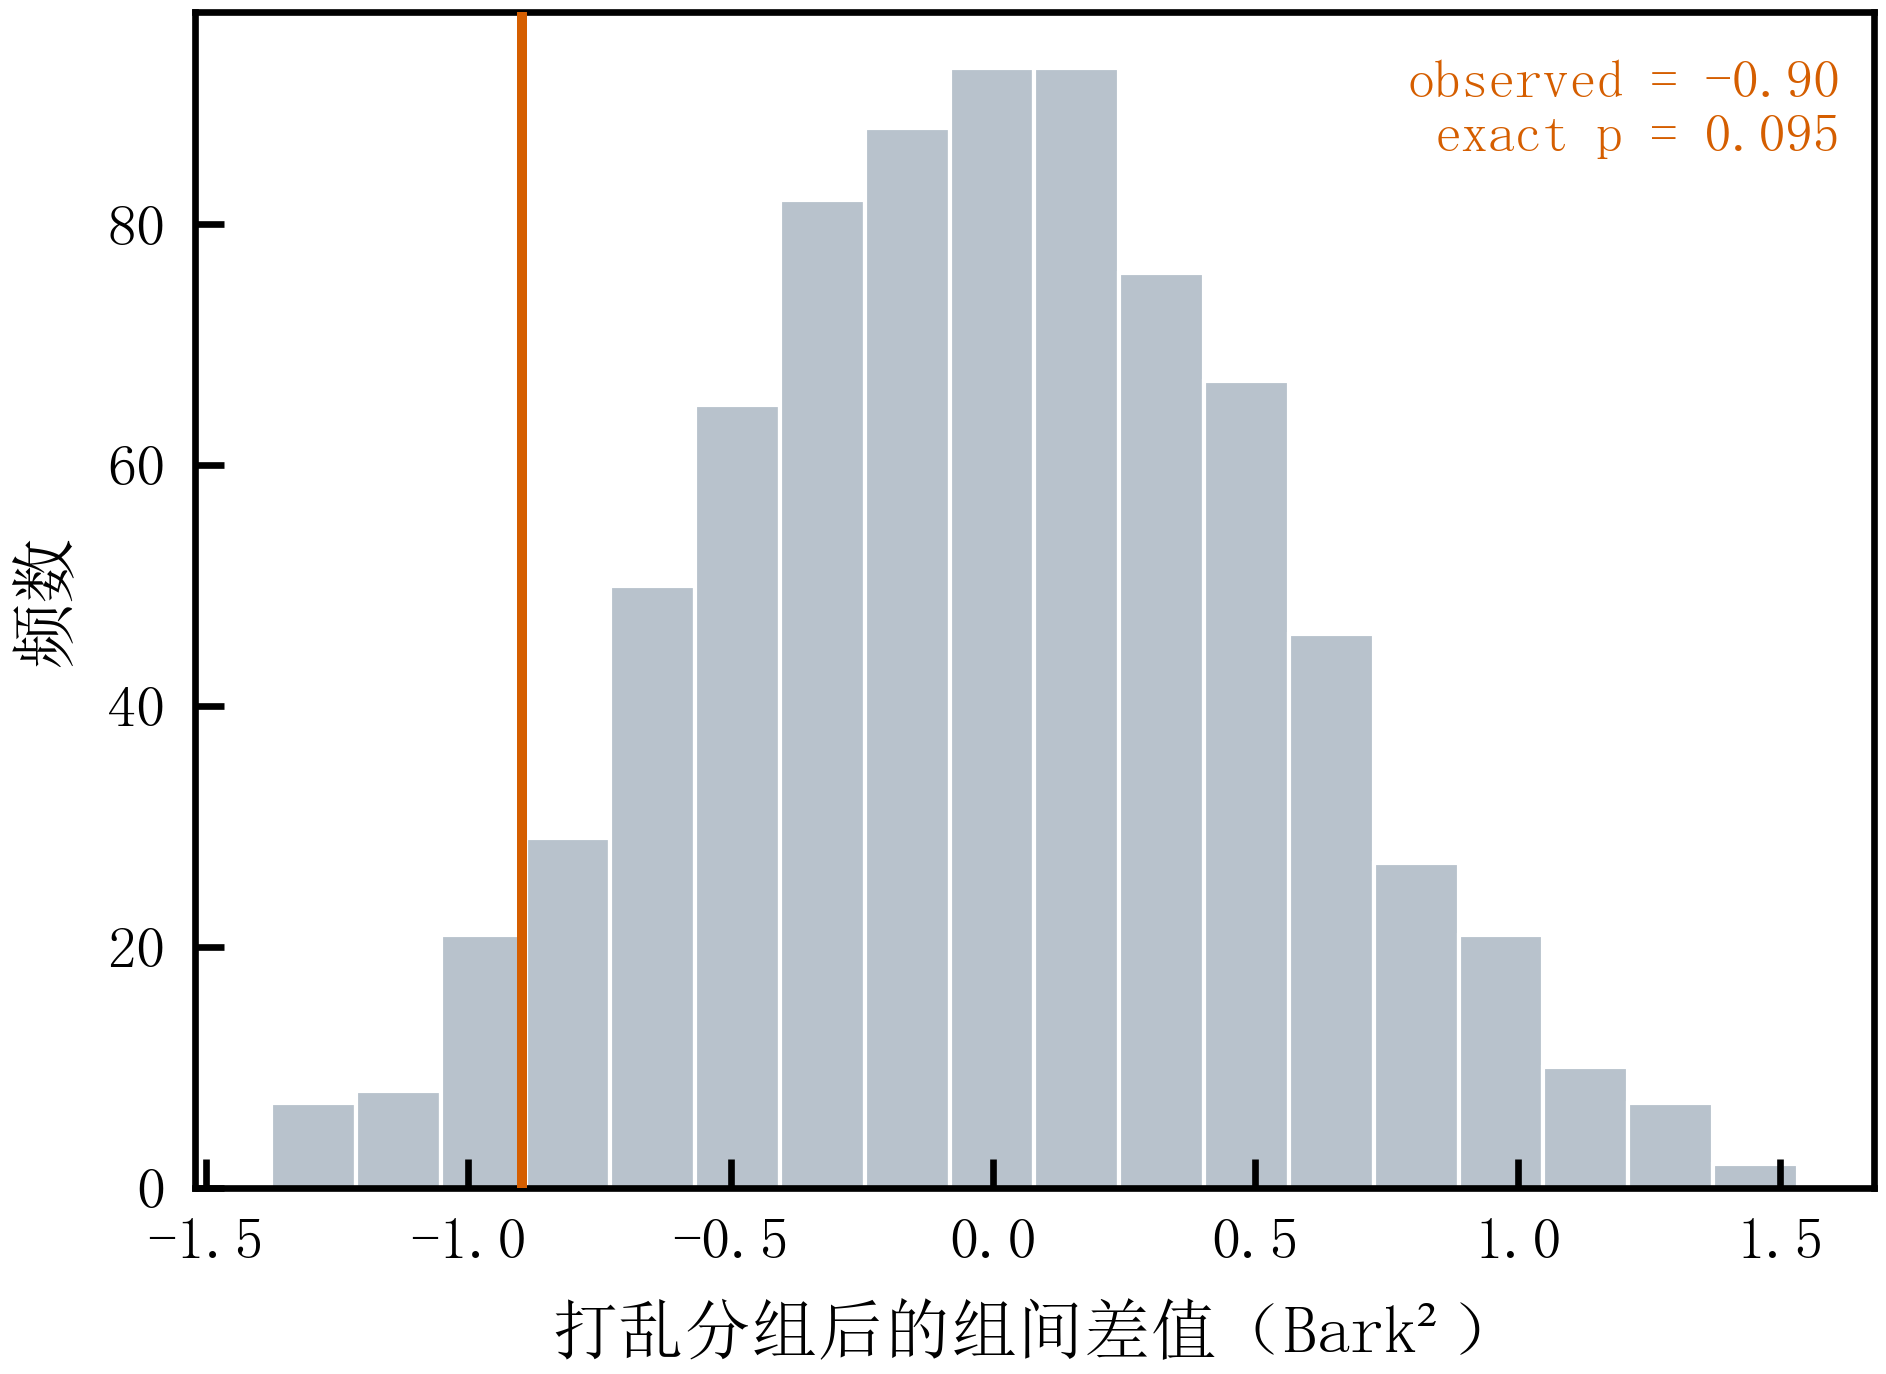
\includegraphics[width=0.62\textwidth]{fig4_permutation.png}
\caption{元音空间面积的精确置换检验。对 12 位说话人的分组标签做全部
$\binom{12}{5}=792$ 种重排得到零分布，红竖线为观测差值，双侧精确 $p=0.095$。}
\label{fig:vsa-perm}
\end{figure}

\subsection{元音对距离}

\begin{table}[htbp]
\centering
\caption{关键元音对的声学距离（归一化 Bark）}
\label{tab:pair}
\begin{tabular}{lcccc}
\toprule
元音对 & 学习者 & 母语者 & 差值 & Cohen's $d$ \\
\midrule
\ipa{ɑː}–\ipa{ʌ} & 0.42 & 0.99 & $-0.57$ & $\mathbf{-3.83}$ \\
\ipa{ɪ}–\ipa{iː} & 0.41 & 1.19 & $-0.79$ & $\mathbf{-2.43}$ \\
\ipa{ʊ}–\ipa{uː} & 0.44 & 0.78 & $-0.35$ & $-1.17$ \\
\ipa{æ}–\ipa{e}  & 0.56 & 0.41 & $+0.15$ & $0.69$ \\
\bottomrule
\end{tabular}
\end{table}

整体指标不显著、局部指标效应极大——这一对比本身即是结论：
\textbf{用元音空间面积做二语语音研究，会漏掉真实效应。}

\begin{figure}[htbp]
\centering
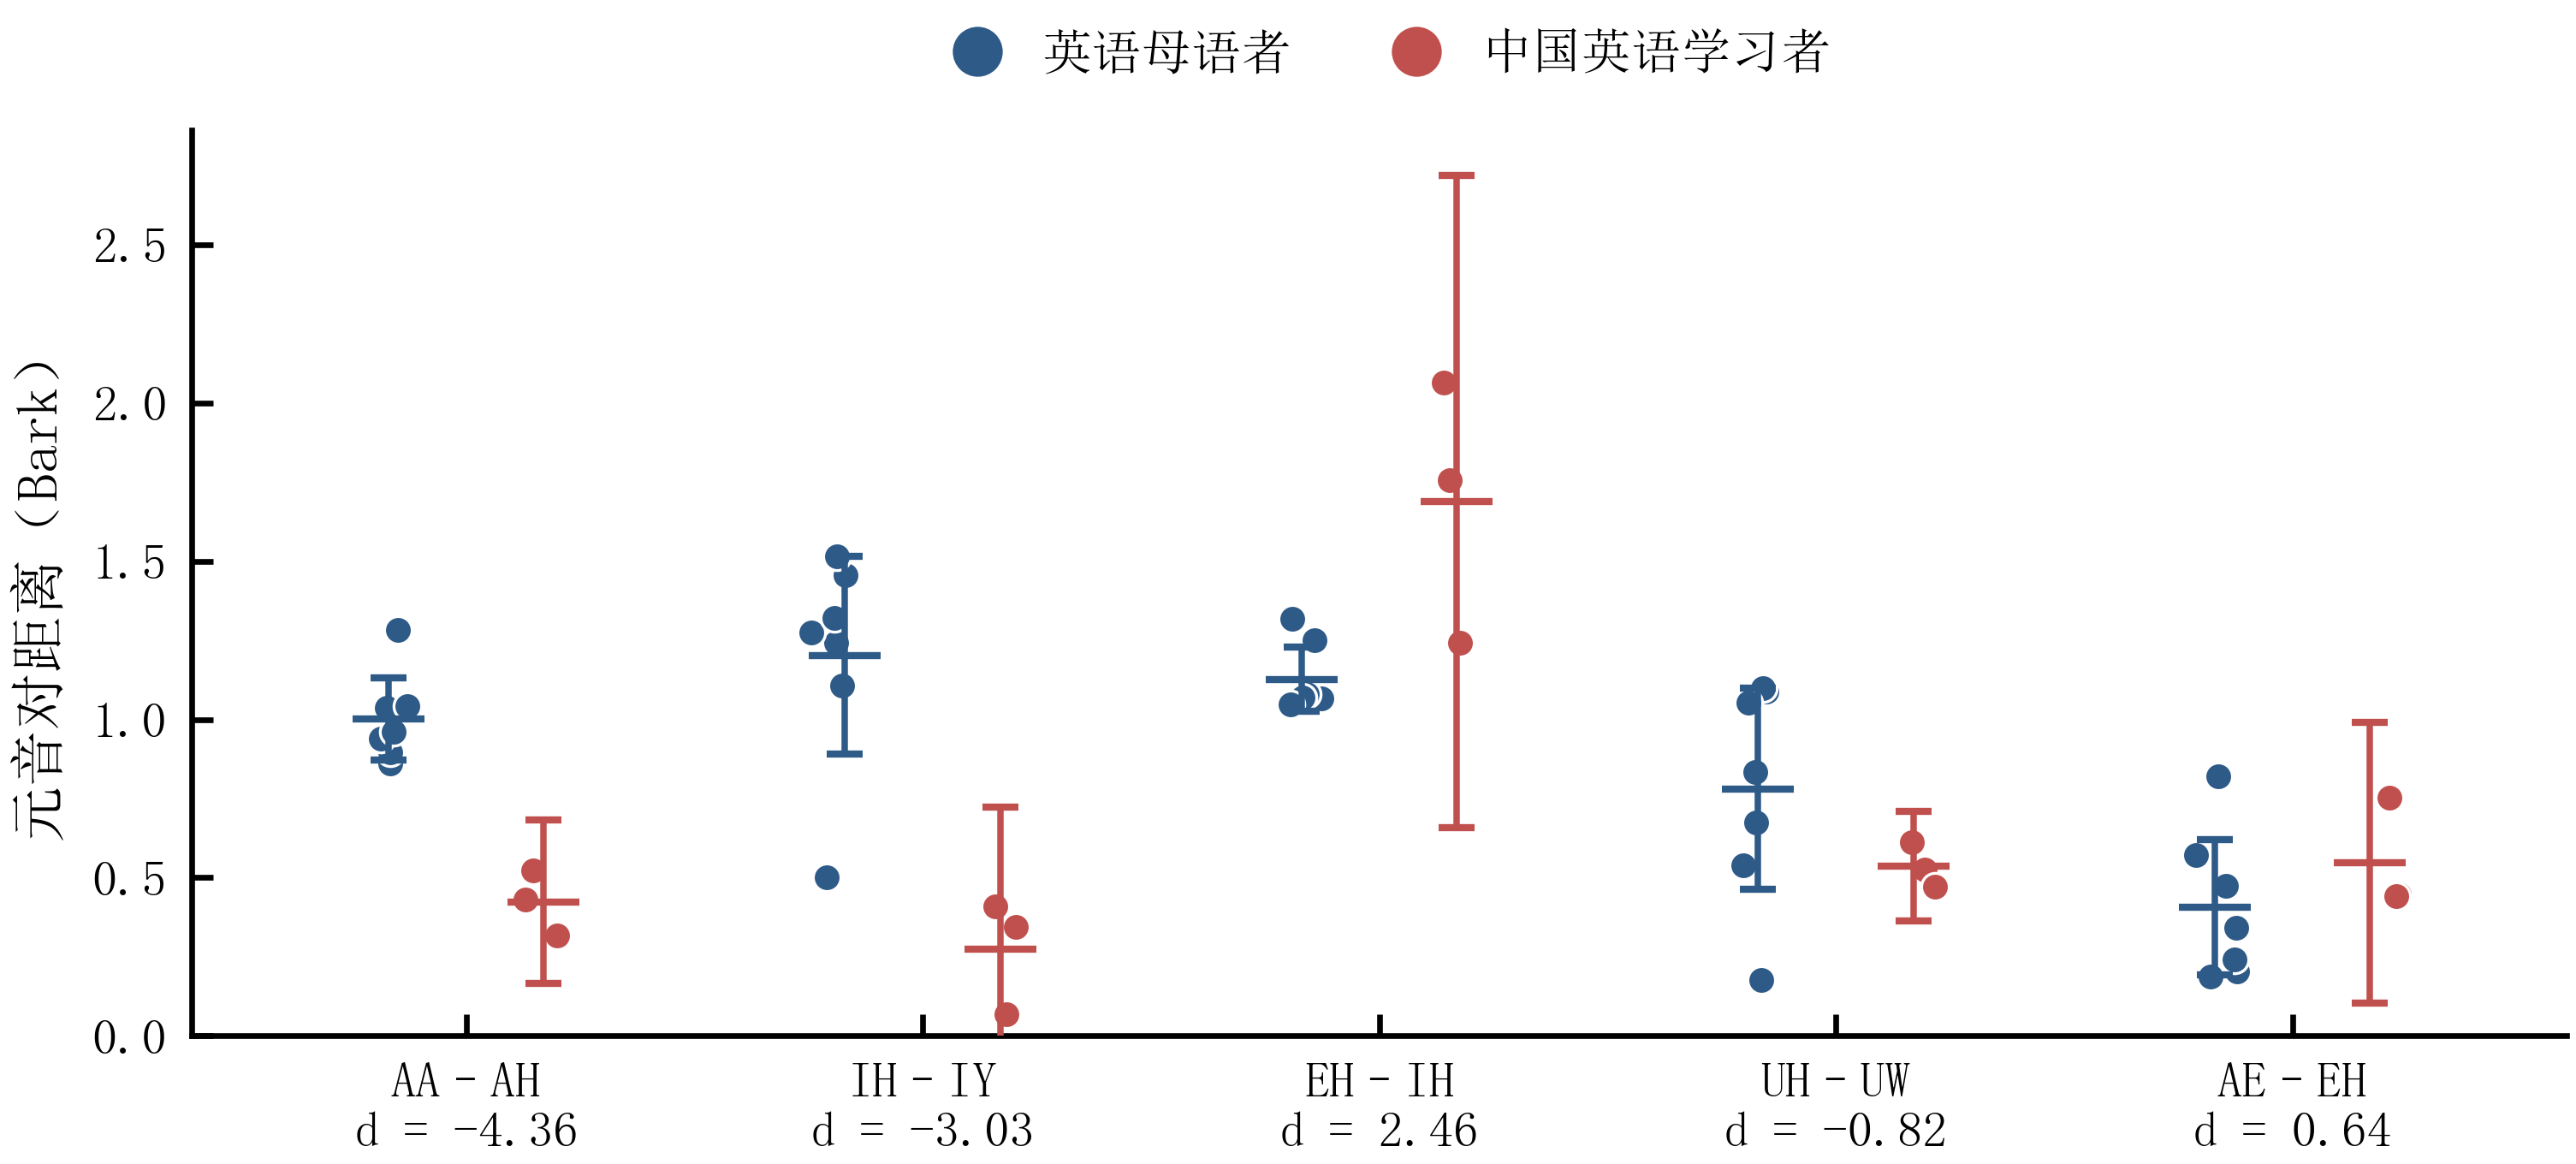
\includegraphics[width=0.95\textwidth]{fig2_pair_distances.png}
\caption{关键元音对的声学距离。每点一位说话人，横线为组均值，误差线为 95\% 置信区间，
按 $|d|$ 降序排列。}
\label{fig:pair}
\end{figure}

\begin{figure}[htbp]
\centering
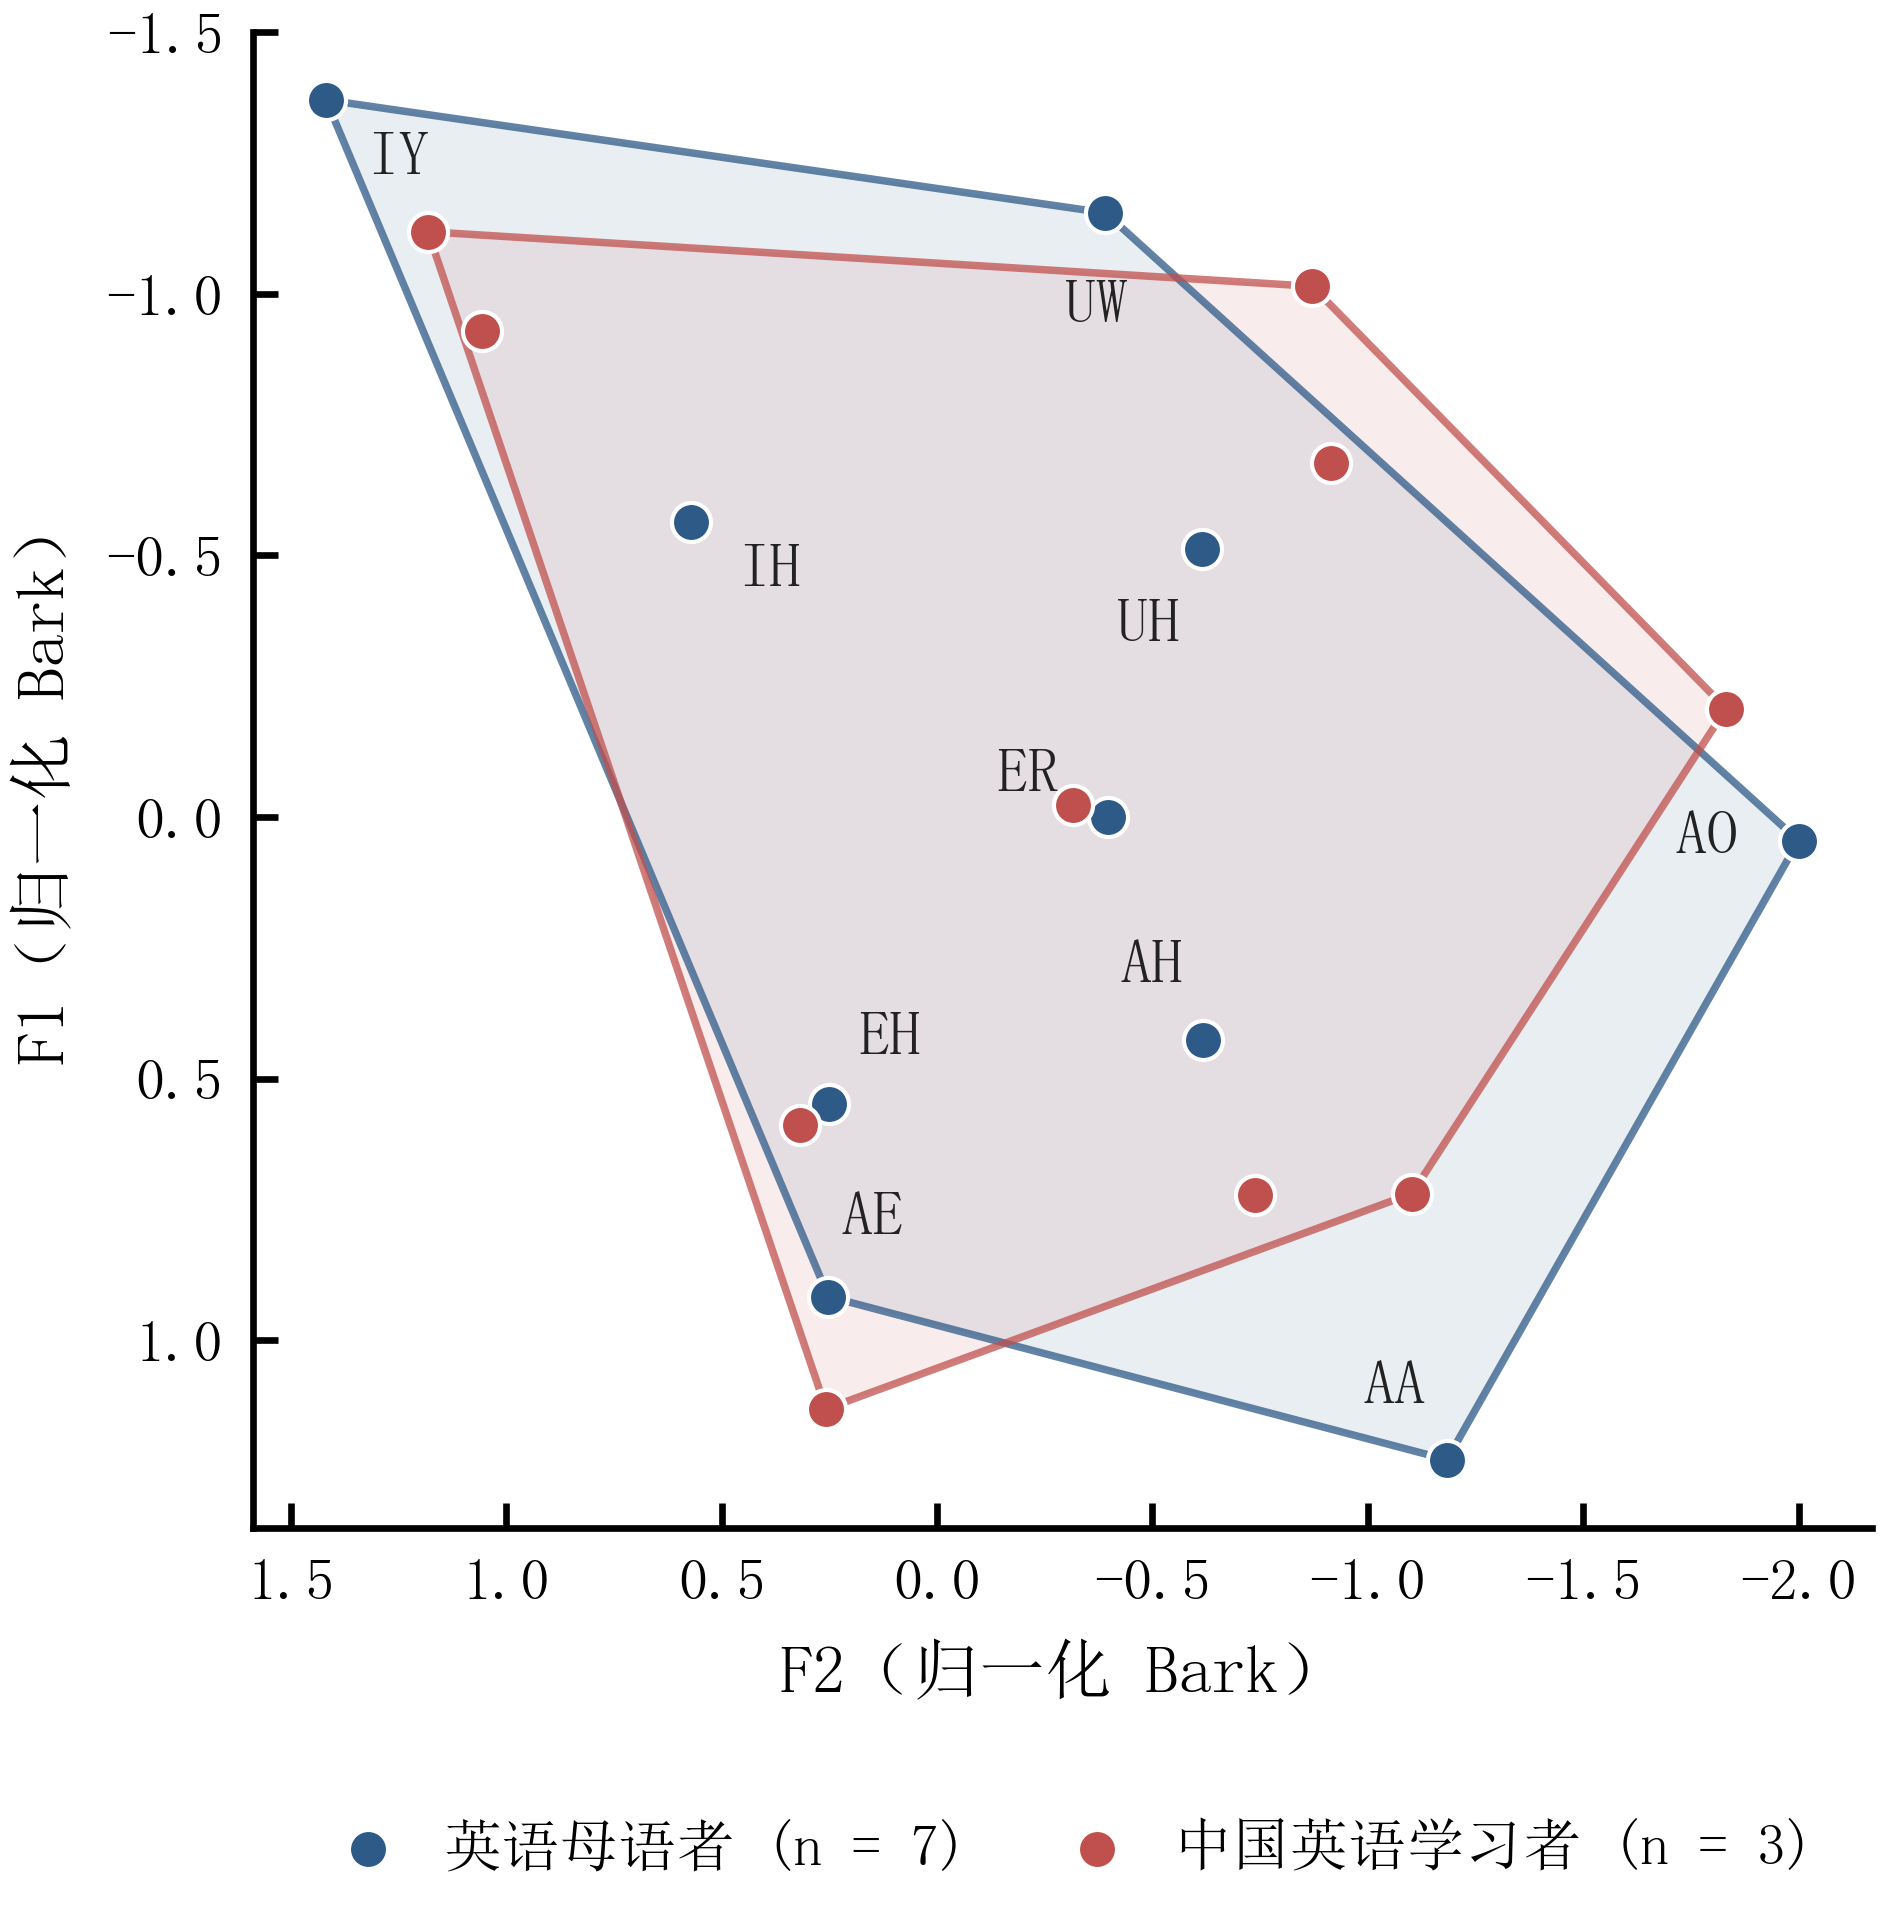
\includegraphics[width=0.60\textwidth]{fig1_vowel_space.png}
\caption{两组元音空间叠加（归一化 Bark）。圆点为英语母语者（$n=7$），三角为普通话学习者
（$n=5$），阴影为凸包。可观察到学习者的 \ipa{ɪ} 明显向 \ipa{iː} 靠拢。}
\label{fig:space}
\end{figure}

\subsection{跨母语比较}

这是本研究的核心结果。七组说话者的 \ipa{ɪ}–\ipa{iː} 距离如下：

\begin{table}[htbp]
\centering
\caption{不同母语背景的 \ipa{ɪ}–\ipa{iː} 距离}
\label{tab:l1}
\begin{tabular}{lccl}
\toprule
组别 & $n$ & 均值 & 备注 \\
\midrule
英语母语者 & 7 & 1.19 & 参照 \\
印地语 & 4 & 0.82 & \\
阿拉伯语 & 4 & 0.81 & \\
韩语 & 4 & 0.41 & \\
\textbf{普通话} & \textbf{5} & \textbf{0.41} & 处于二语组中间位置 \\
西班牙语 & 4 & 0.24 & 合并更严重 \\
越南语 & 3 & 0.16 & 合并最严重 \\
\bottomrule
\end{tabular}
\end{table}

\begin{table}[htbp]
\centering
\caption{组间检验}
\label{tab:l1-test}
\begin{tabular}{llc}
\toprule
比较 & 统计量 & 结果 \\
\midrule
七组整体差异 & Kruskal--Wallis & $H=20.82$，$p=0.002$ \\
普通话 vs 英语母语者 & Mann--Whitney & $d=-2.43$，$p=0.005$ \\
其他二语组 vs 英语母语者 & Mann--Whitney & $d=-1.96$，$p<0.001$ \\
\textbf{普通话 vs 其他二语组} & Mann--Whitney & $\bm{d=-0.29}$，$\bm{p=0.73}$ \\
仅六个二语组之间 & Kruskal--Wallis & $H=12.75$，$p=0.026$ \\
\bottomrule
\end{tabular}
\end{table}

\begin{figure}[htbp]
\centering
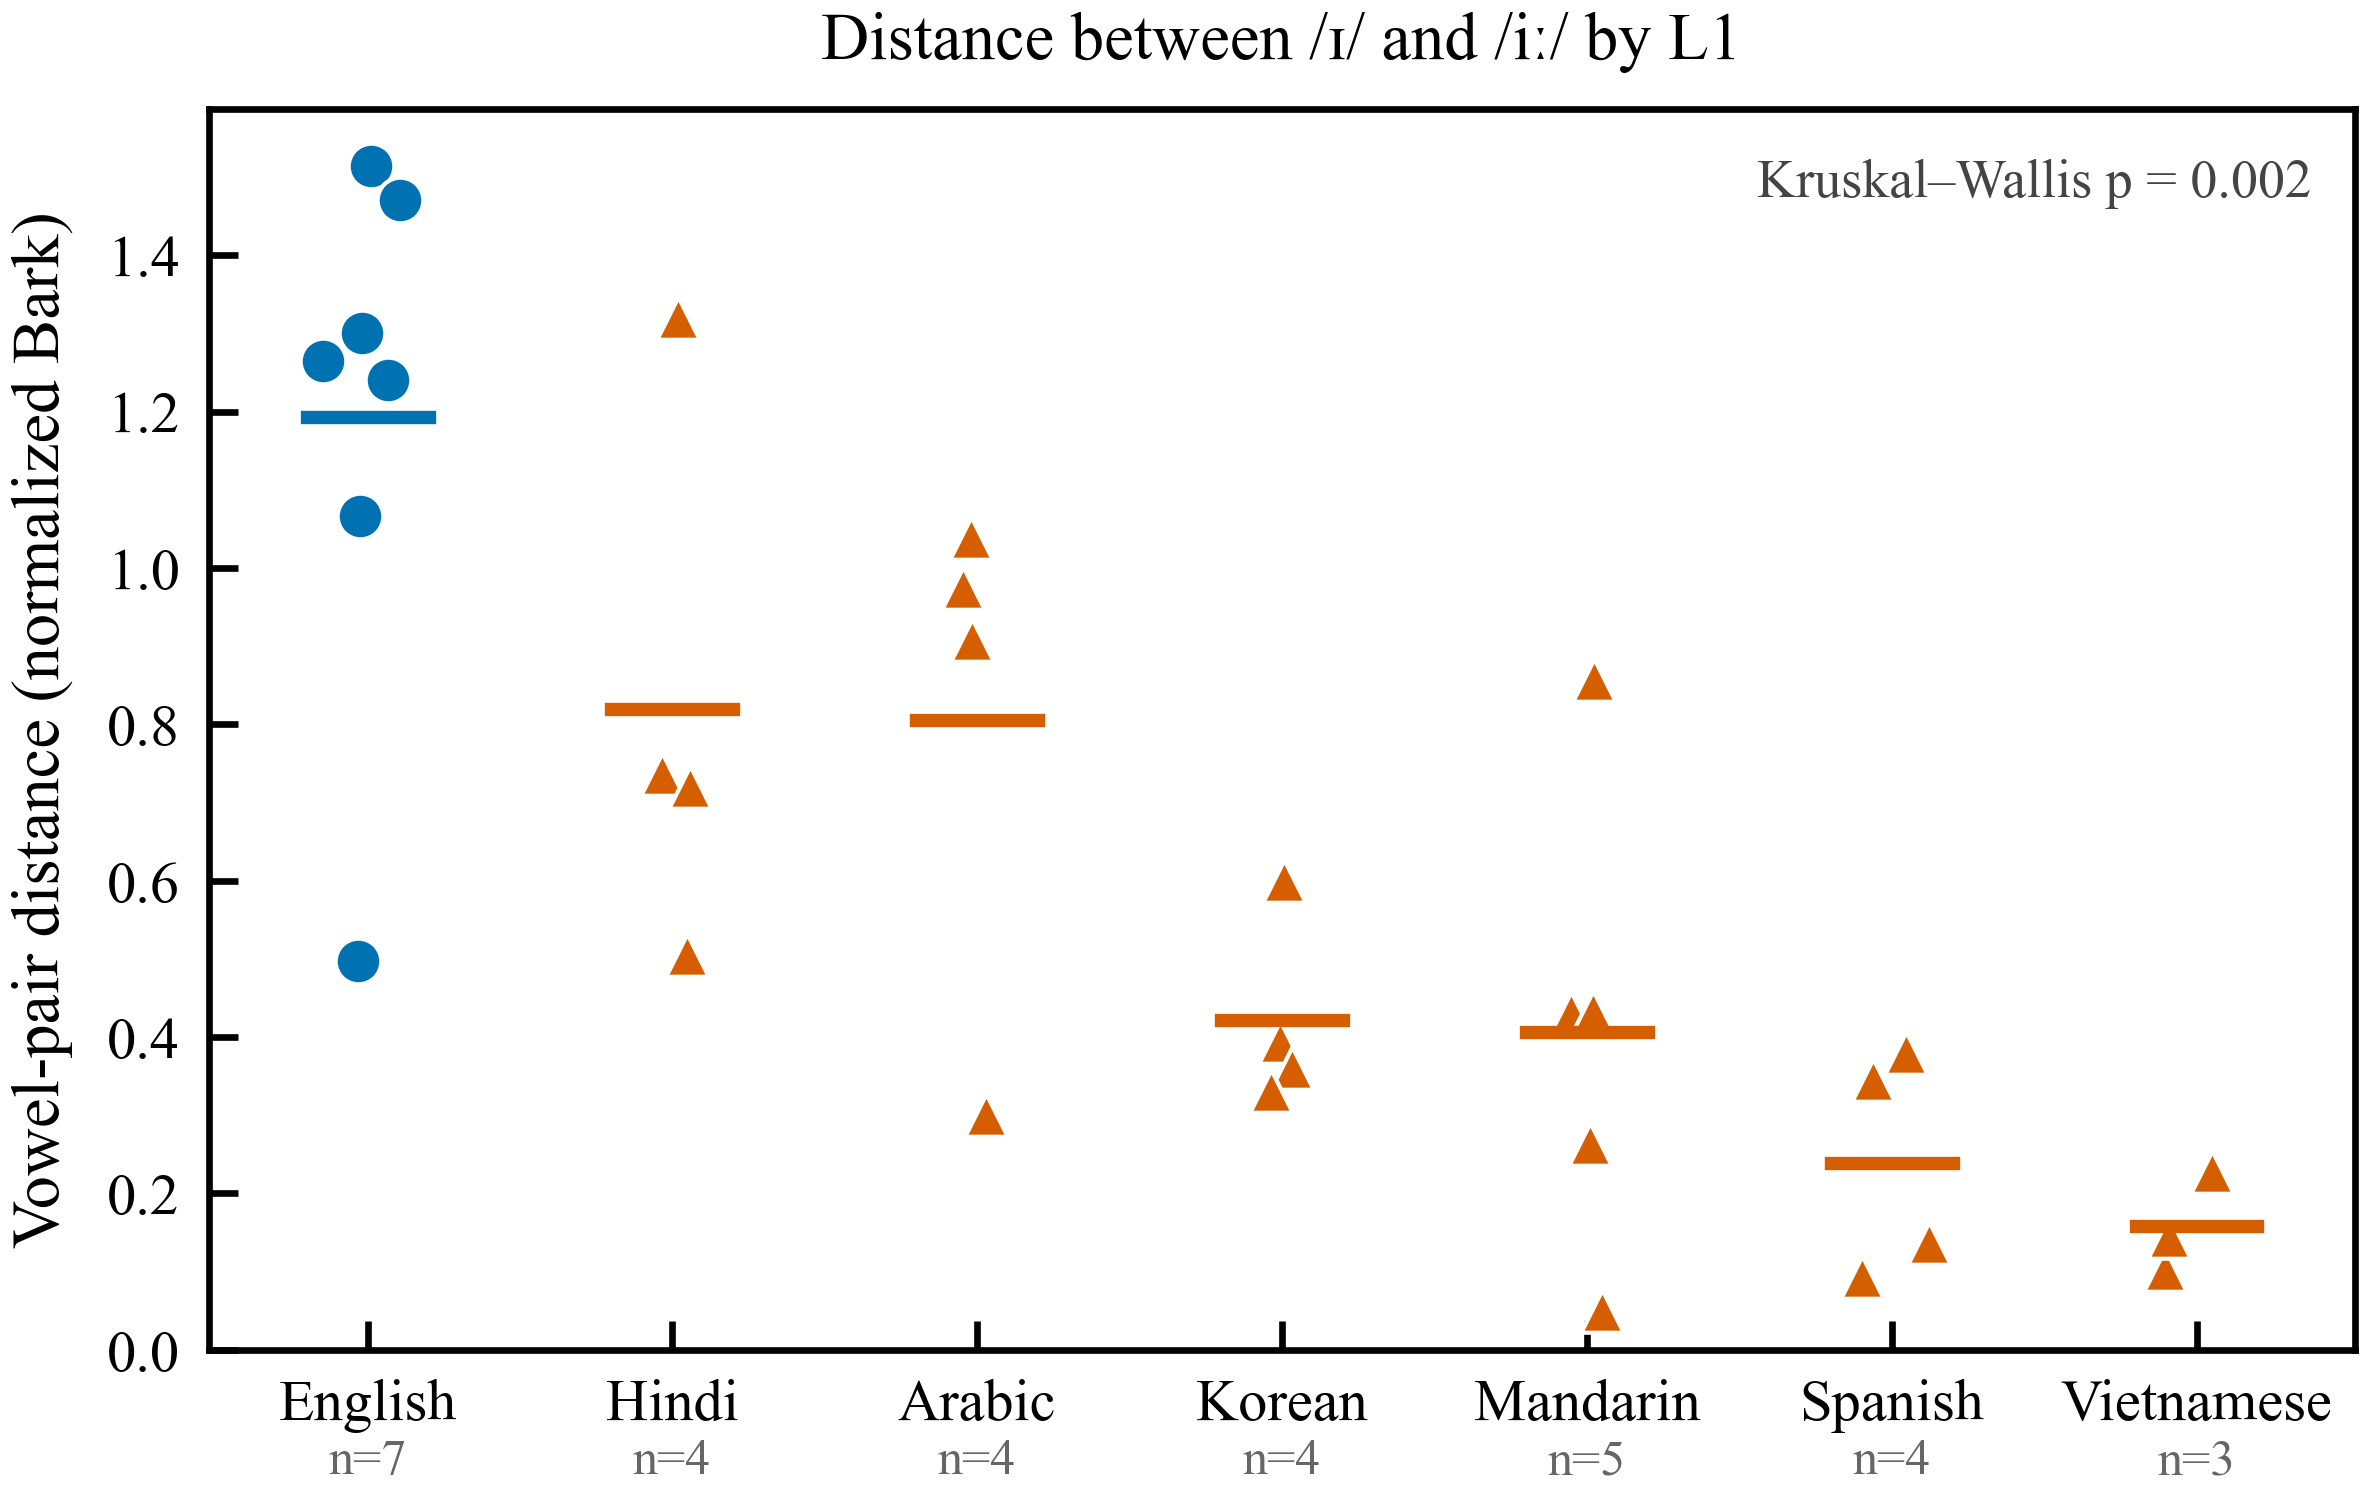
\includegraphics[width=0.88\textwidth]{fig8_l1_comparison.png}
\caption{不同母语背景的 \ipa{ɪ}–\ipa{iː} 距离。每点一位说话人，横线为组均值，
按均值降序排列。普通话与其他二语组无显著差异（$p=0.73$）。}
\label{fig:l1}
\end{figure}

\textbf{结论：\ipa{ɪ}–\ipa{iː} 的范畴合并是二语学习的普遍困难，不是某一母语特有的迁移。}
西班牙语、越南语的合并程度甚至强于普通话；普通话在二语组中处于中间位置。
各组之间确有显著差异（$p=0.026$），说明母语背景具有调节作用，但"普通话缺少松紧对立"
这一条无法解释整体格局。

\subsection{时长与语速}

\begin{table}[htbp]
\centering
\caption{时长与语速}
\label{tab:dur}
\begin{tabular}{lccc}
\toprule
指标 & 学习者 & 母语者 & 效应量 \\
\midrule
\ipa{iː}:\ipa{ɪ} 时长比（重读） & 1.13 & 1.27 & $d=-1.06$，$p=0.074$ \\
语速（音节/秒） & 2.89 & 3.64 & $d=-2.51$，$p=0.005$ \\
\bottomrule
\end{tabular}
\end{table}

时长方面学习者确实拉得不够长，但未达显著，作为\textbf{趋势}报告。
按母语背景看，印地语（1.33）与阿拉伯语（1.31）几乎保持了母语者的时长对比，
而普通话（1.13）、韩语（1.16）、西班牙语（1.03）没有。

\begin{figure}[htbp]
\centering
\begin{minipage}{0.48\textwidth}
  \centering
  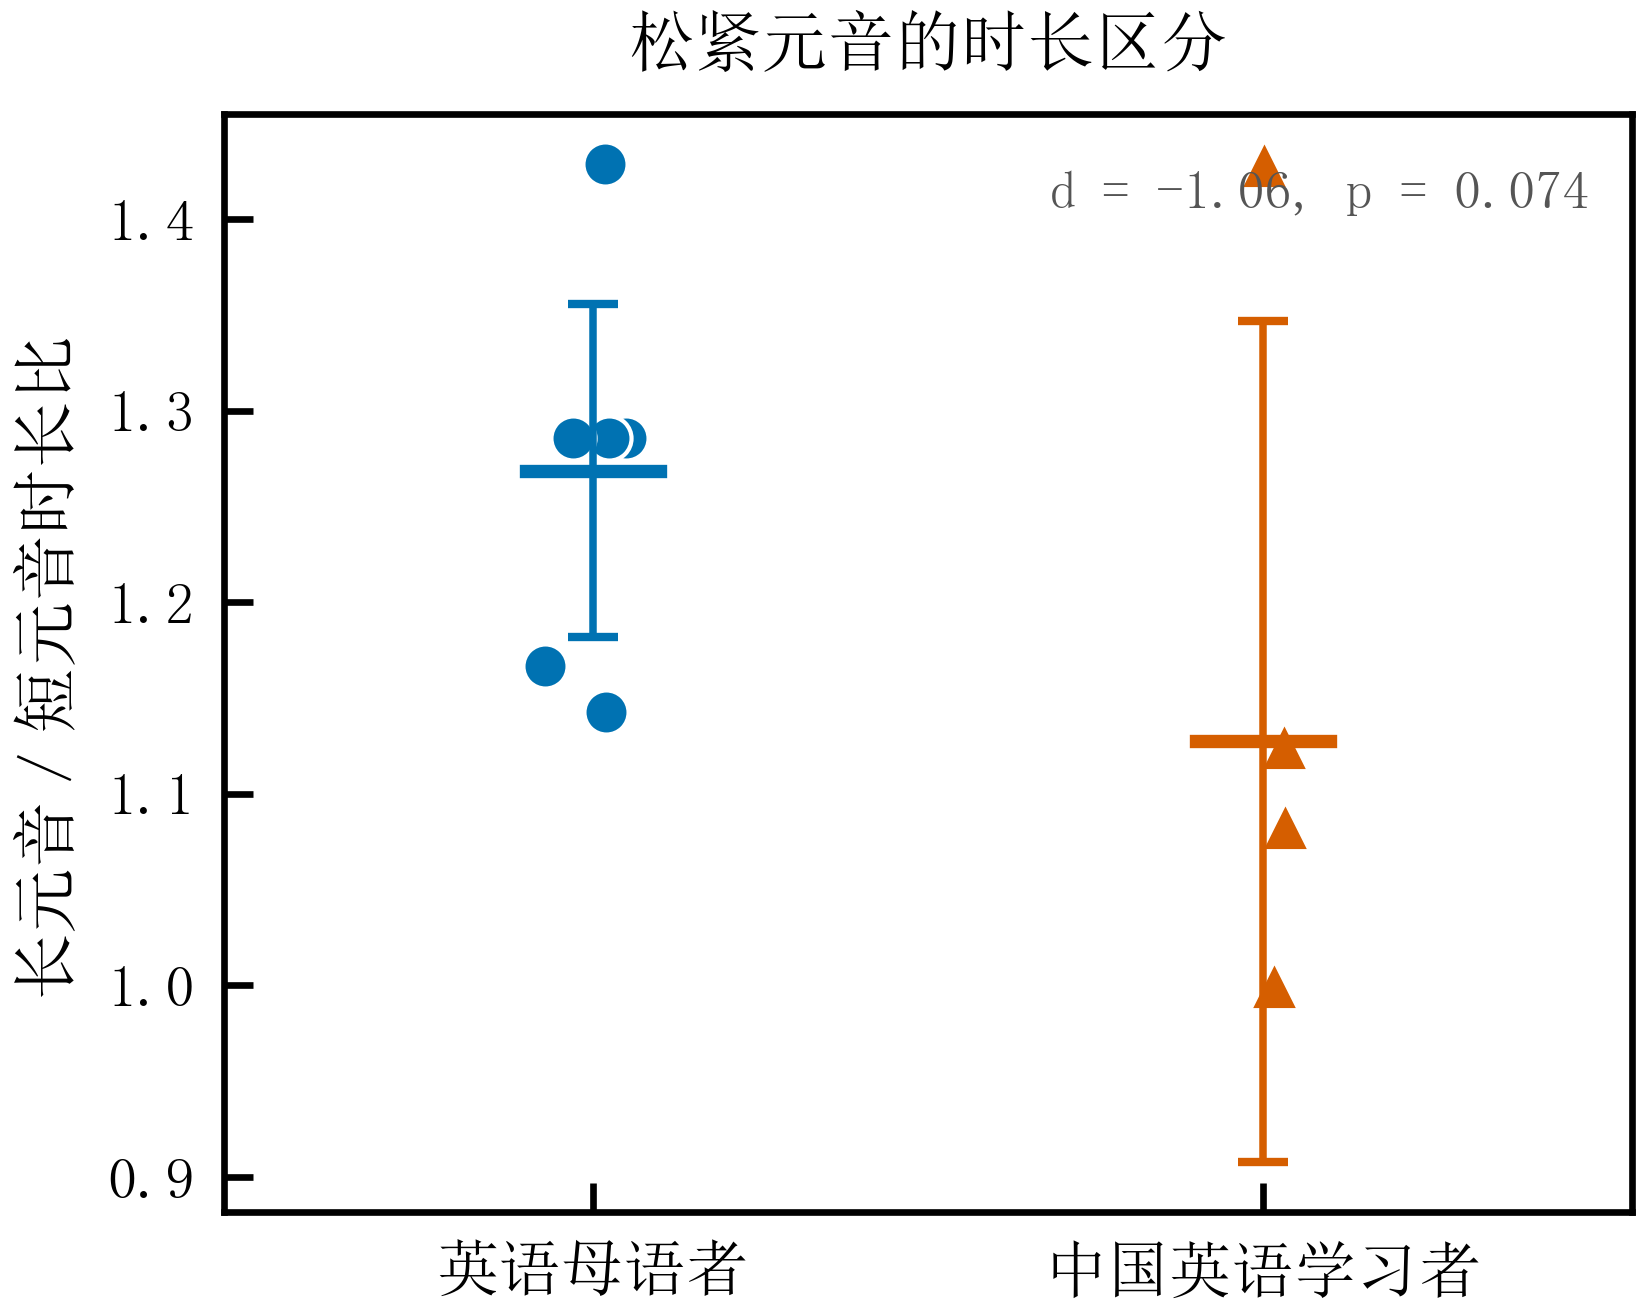
\includegraphics[width=\textwidth]{fig6_duration.png}
  \caption{松紧元音的时长区分}
  \label{fig:dur}
\end{minipage}\hfill
\begin{minipage}{0.48\textwidth}
  \centering
  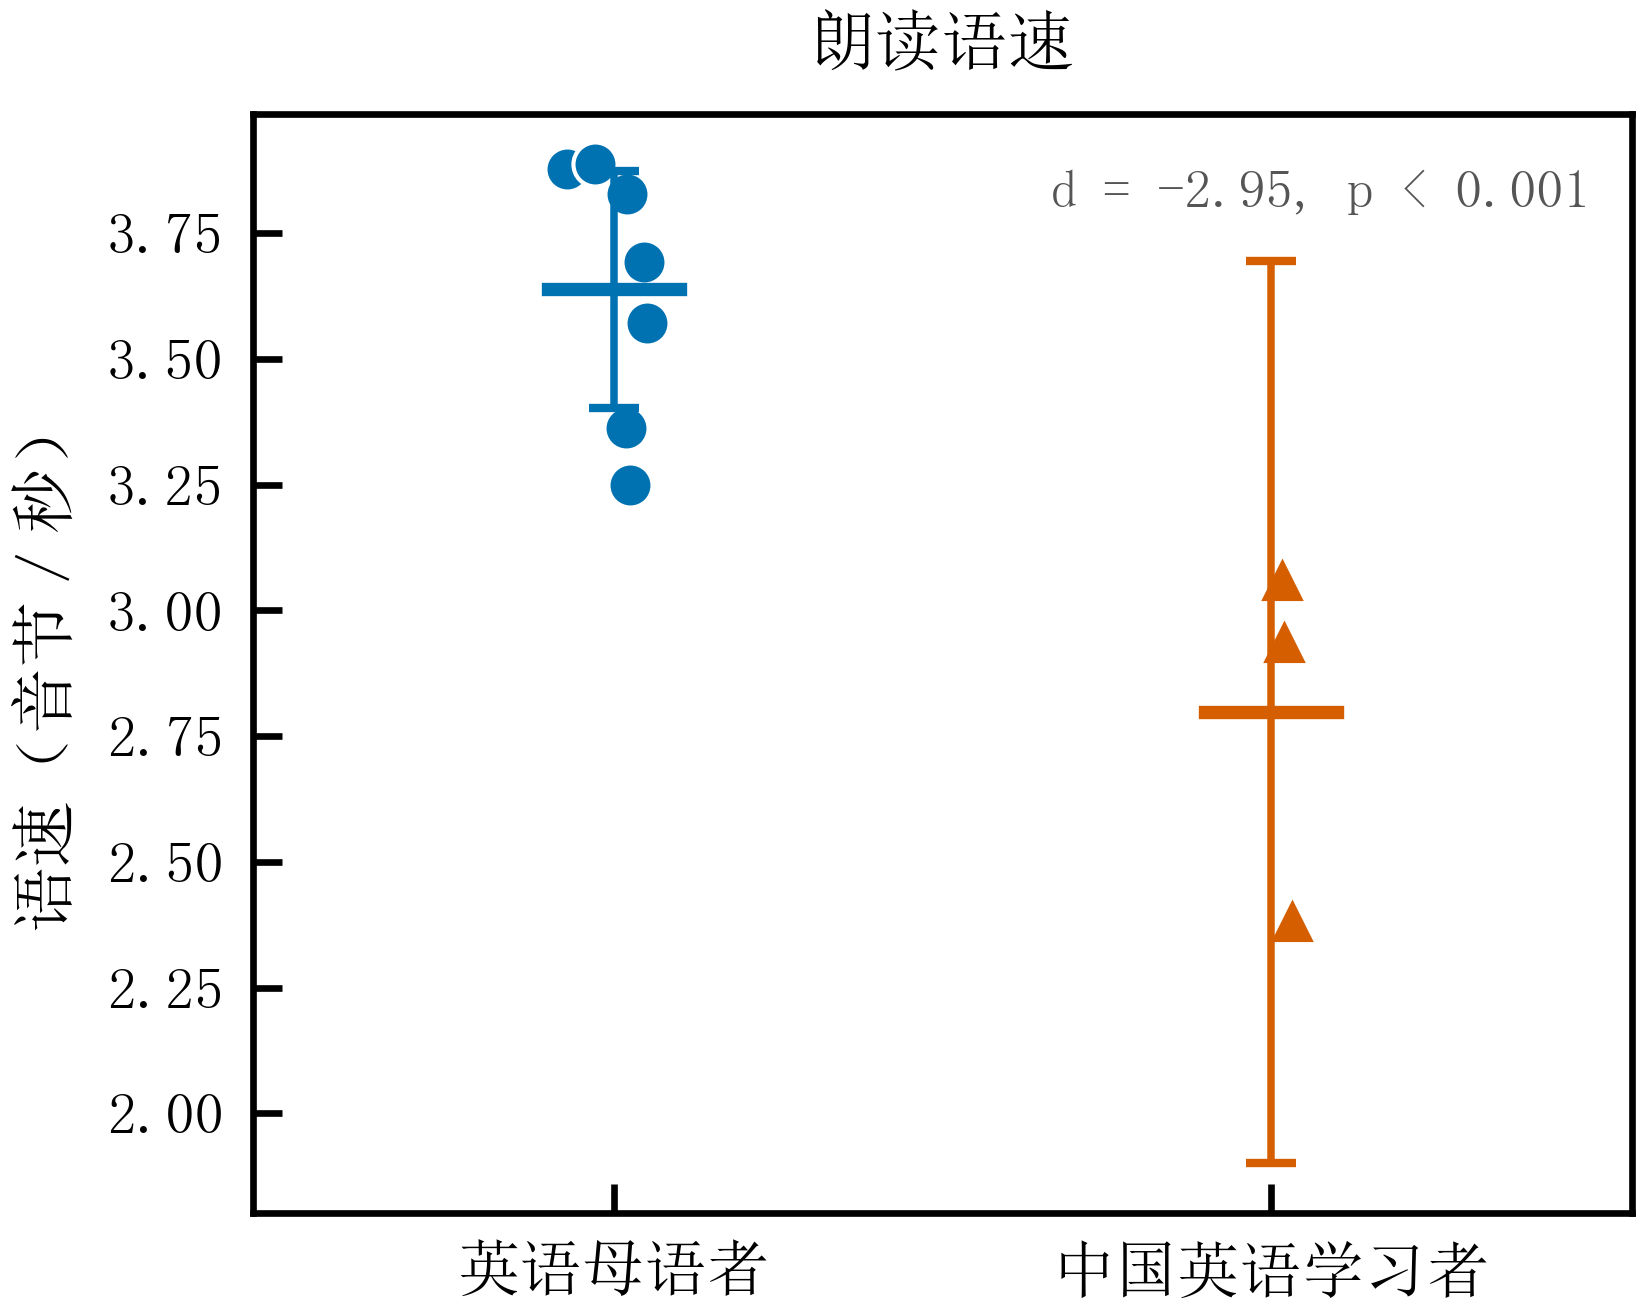
\includegraphics[width=\textwidth]{fig7_rate.png}
  \caption{朗读语速}
  \label{fig:rate}
\end{minipage}
\end{figure}

\subsection{混合效应模型}

模型 $F_1 \sim \text{group}\times\text{vowel} + \text{gender} + (1\mid\text{speaker})$
（普通话 vs 母语者，16{,}586 个 token）。组别主效应不显著，但多个元音的组×元音交互项显著，
说明差异是局部的（\figref{fig:forest}）。

\begin{figure}[htbp]
\centering
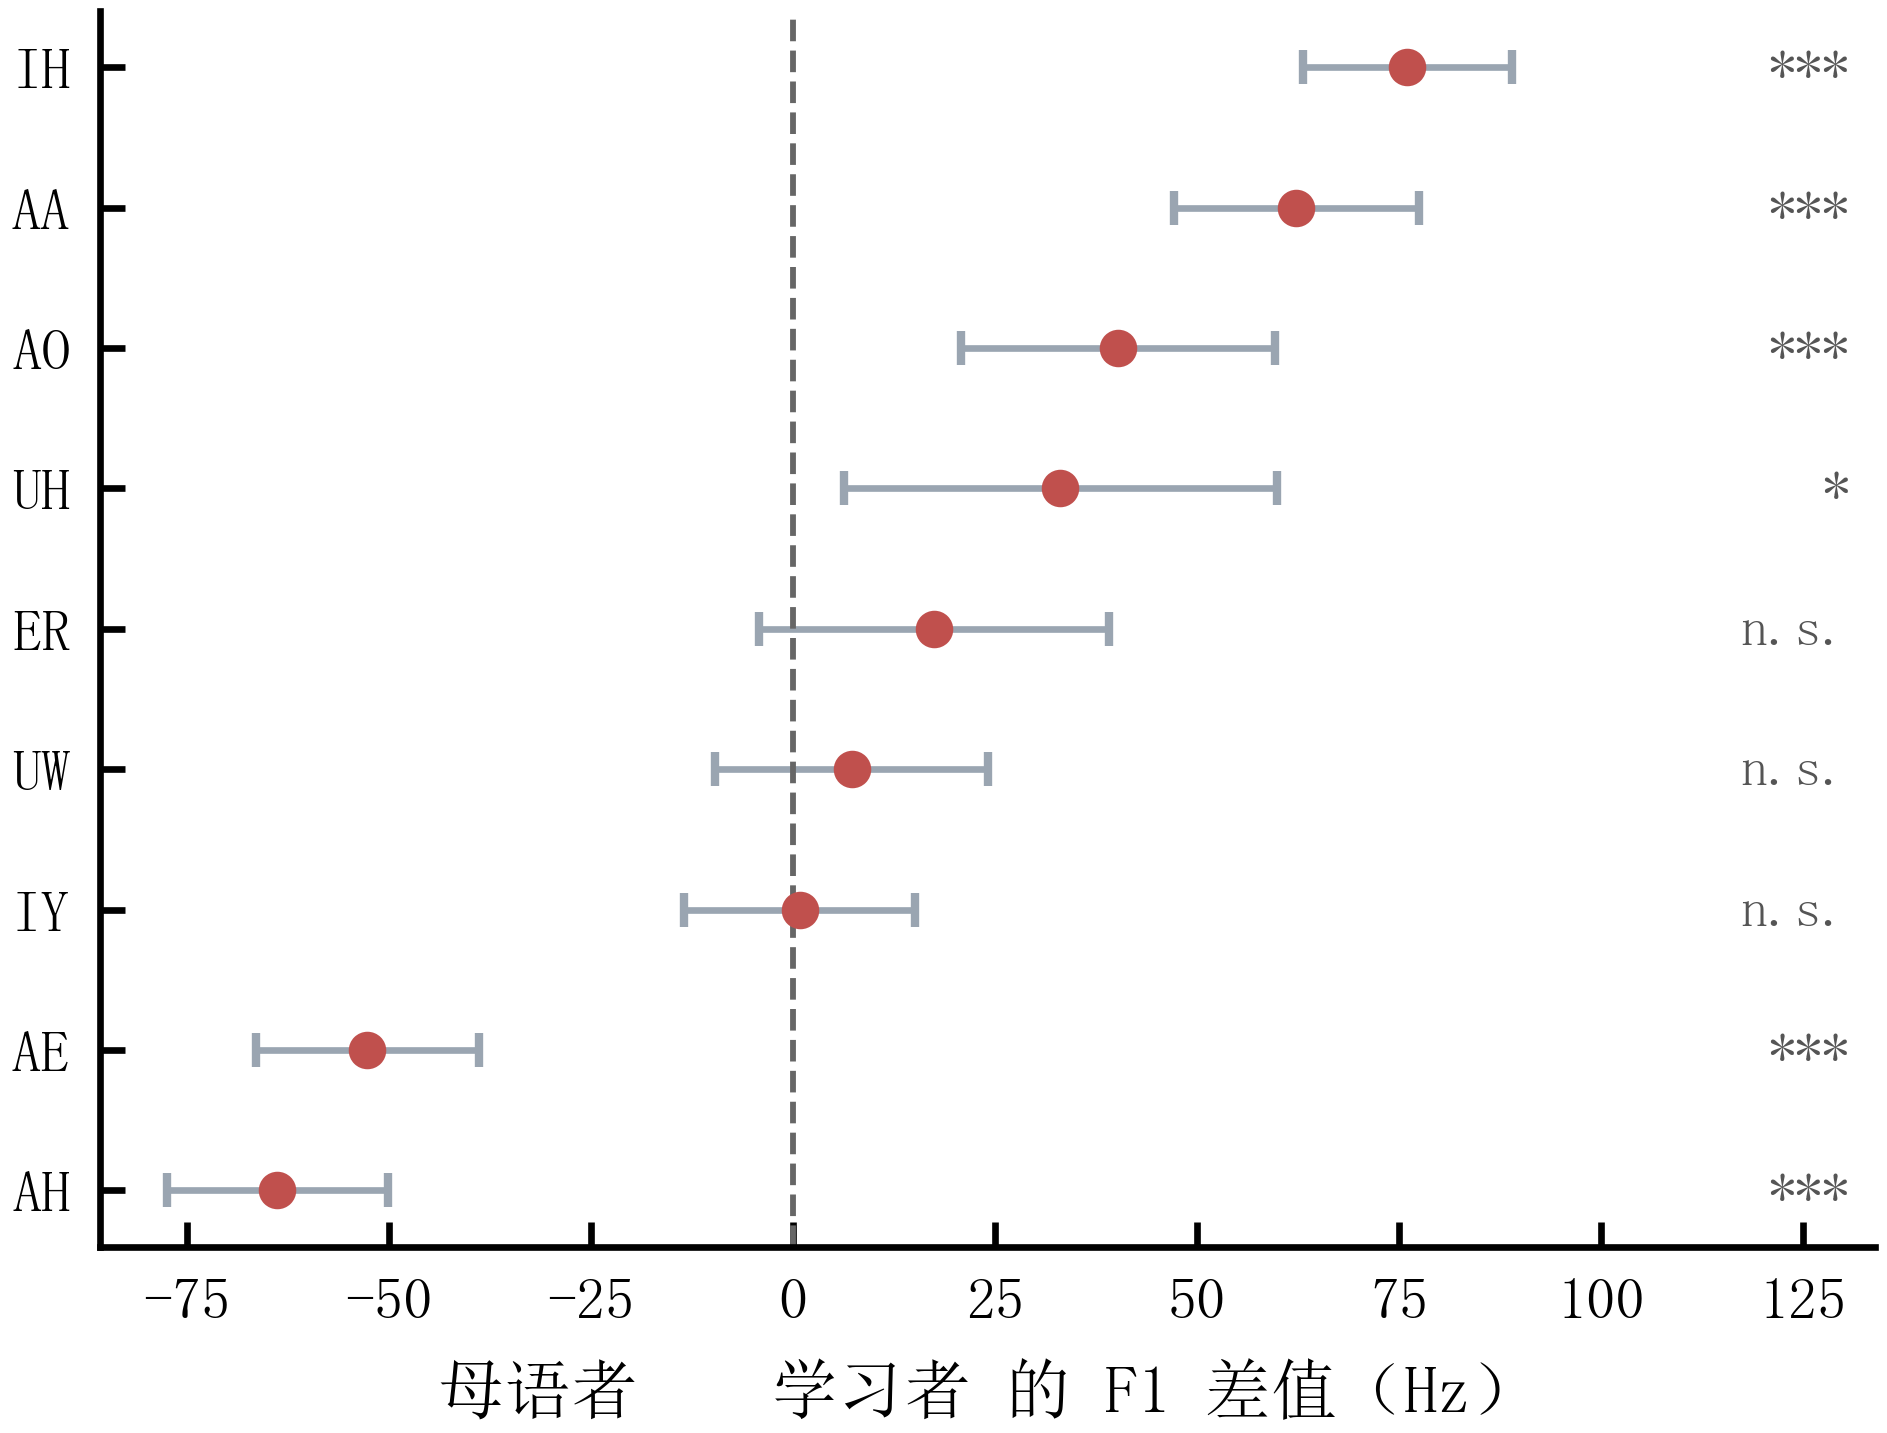
\includegraphics[width=0.62\textwidth]{fig3_forest.png}
\caption{混合效应模型的组别×元音交互项。点为母语者相对学习者的 F1 差值，
误差线为 95\% 置信区间。}
\label{fig:forest}
\end{figure}

\subsection{可懂度验证}

\begin{table}[htbp]
\centering
\caption{ASR 词错率与元音偏离度的关系}
\label{tab:wer}
\begin{tabular}{lccc}
\toprule
组别 & $n$ & 平均 WER & 与元音偏离的 Spearman $\rho$ \\
\midrule
中国学习者 & 5 & 24.0\% & \multirow{2}{*}{0.937（全体 12 人，$p<0.001$）} \\
英语母语者 & 7 & 7.7\% & \\
\midrule
仅母语者 & 7 & 7.7\% & 1.000（$p<0.001$） \\
\bottomrule
\end{tabular}
\end{table}

组内同样是完美秩相关，说明这不是"两组不同"造成的假象：即使母语者内部，
元音越偏离标准分布的人被 ASR 听错的也越多。

\begin{figure}[htbp]
\centering
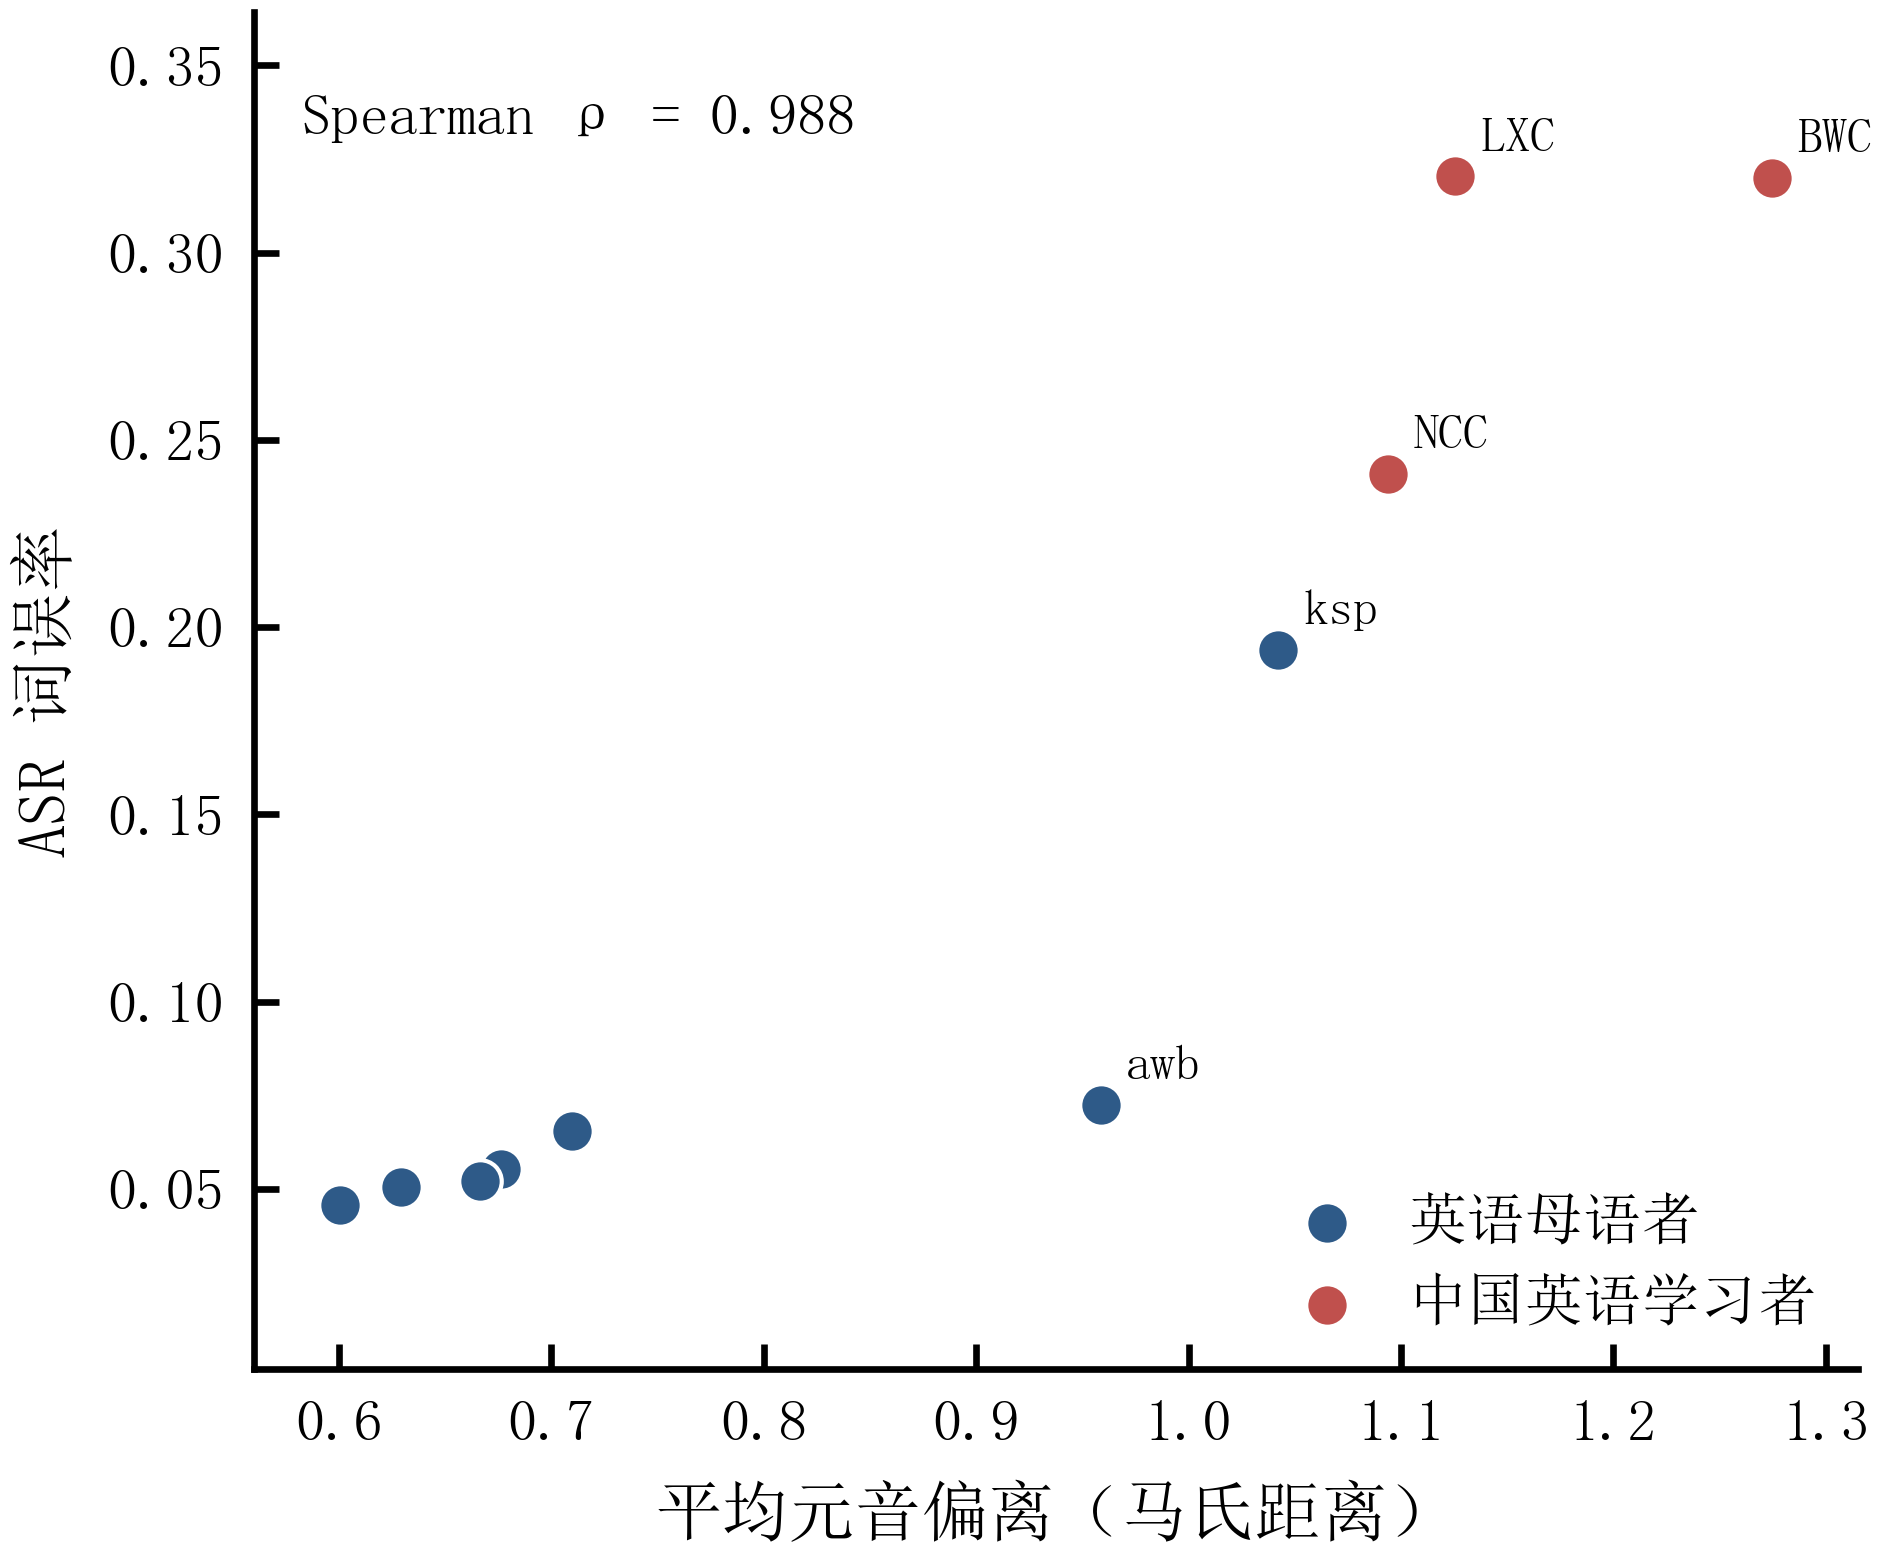
\includegraphics[width=0.60\textwidth]{fig5_wer.png}
\caption{元音偏离度与 ASR 词错率。横轴为说话人各元音到母语者参照分布的平均马氏距离，
纵轴为 40 句朗读的词错率。}
\label{fig:wer}
\end{figure}

\subsection{小样本鲁棒性}

标准 Lobanov 依赖说话人自身的均值与方差，短录音时估计噪声大。实测中同一位说话人
12 句给出 \ipa{iː}:\ipa{ɪ} 时长比 1.60，250 句给出 1.14，结论相反。

为此实现了收缩归一化（经验贝叶斯）：

\begin{equation}
\hat{\mu} = \frac{n\mu_s + k\mu_{\text{pop}}}{n+k}, \qquad
\hat{\sigma} = \frac{n\sigma_s + k\sigma_{\text{pop}}}{n+k}
\end{equation}

以 \ipa{ɪ}–\ipa{iː} 距离的稳定性为指标（重复抽样 40 次，与全样本结果比较）：

\begin{table}[htbp]
\centering
\caption{小样本下两种归一化的稳定性}
\label{tab:shrink}
\begin{tabular}{cccc}
\toprule
token 数 & 标准 Lobanov 偏差 & 收缩法偏差 & 改进 \\
\midrule
10 & 0.409 & 0.380 & 7.1\% \\
20 & 0.324 & 0.311 & 3.9\% \\
30 & 0.266 & 0.260 & 2.2\% \\
50 & 0.199 & 0.195 & 1.8\% \\
\bottomrule
\end{tabular}
\end{table}

\textbf{改进有限（4--7\%）。} 原因推测：先验取自母语者，而学习者系统性地偏离母语者分布，
收缩会同时把偏差拉进来。这是一个诚实的负结果，本研究不宣称"解决了小样本问题"。

\subsection{负结果：擦音频谱矩}

\ipa{θ}/\ipa{ð} 的频谱矩曾实现并分析，三条独立检验均未通过：组间差异 $p=0.25$；
ASR 在含 th 词上的错误率与非 th 词无差异；频谱重心与 th 词错误率无关（$\rho=-0.04$）；
且同一说话人 \ipa{θ} 与 \ipa{f} 的重心关系都不稳定。

故未纳入诊断工具，也未纳入图集。这一负结果说明：不是所有可测的量都值得做成诊断指标，
必须有独立的效度证据。

% =====================================================================
\section{诊断工具的实现}

\subsection{系统结构}

\begin{table}[htbp]
\centering
\caption{工具的处理流程}
\label{tab:pipeline}
\begin{tabular}{ll}
\toprule
步骤 & 说明 \\
\midrule
1. 音素级对齐 & MFA \texttt{align\_one}，单文件约 20--80 秒 \\
2. 共振峰提取 & 元音中段 50\% 窗口，LPC 每 5 ms 估计，取中位数 \\
3. 归一化 & 说话人内 Lobanov（Bark 标度） \\
4. 评分 & 与母语者参照分布比较的马氏距离，$\chi^2(2)$ 转百分位 \\
5. 输出 & 逐元音得分、问题元音排序、教学建议 \\
\bottomrule
\end{tabular}
\end{table}

\subsection{评分方法}

对每个元音 $v$，以 7 位母语者中位数点的均值 $\mu_v$ 与协方差 $\Sigma_v$ 构成参照分布。
评分定义为

\begin{equation}
d_v = \sqrt{(x_v - \mu_v)^{\top}\Sigma_v^{-1}(x_v-\mu_v)},\qquad
s_v = 100\bigl(1 - F_{\chi^2_2}(d_v^2)\bigr)
\end{equation}

$s_v$ 可解释为"该发音比多少比例的母语者更偏离中心"。公式固定，未做人工调参。

\subsection{使用方式}

命令行：

\begin{verbatim}
python3 src/diagnose.py --wav my.wav --text "the text you read"
\end{verbatim}

网页界面：\texttt{streamlit run src/app.py}。

单次录音建议朗读 30 句以上，否则时长比的估计不稳定（见第 5.8 节）。

% =====================================================================
\section{讨论}

\subsection{为什么整体指标会失效}

元音空间面积把所有元音压缩成一个数。若错误是局部的（少数元音偏移），
面积的平均化会把信号稀释；同时面积对个体差异极为敏感，母语者组内即在 3.45--6.16 之间
波动，远超组间差异。这解释了为什么面积检验只有 $p=0.095$，而元音对距离可达 $d=-3.83$。

对方法学的启示：二语语音研究若只报告 VSA，可能系统性地低估二语者的困难。

\subsection{对母语迁移解释的修正}

本研究的起点假设是"普通话没有英语的松紧元音对立，因此学习者把 \ipa{ɪ} 与 \ipa{iː}
合并为一个范畴"。若该假设成立，合并应主要集中在普通话组。

数据不支持这一预测：六种母语背景全部出现合并，西班牙语与越南语更强，普通话与其余二语组
无差异（$p=0.73$）。这说明该困难更可能源于二语感知与产出的普遍机制
（如范畴边界重建的困难、输入中对立线索的统计分布），而非单一母语的音位库存。

需要说明的是，这并非否定母语迁移的存在：组间差异仍然显著（$p=0.026$），
说明母语背景有调节作用，只是它不是主导因素。

\subsection{教学含义}

\begin{enumerate}[leftmargin=2em,itemsep=2pt]
  \item 训练应优先针对\textbf{具体元音对}，而非笼统地"改善发音"。本研究中
        \ipa{ɑː}–\ipa{ʌ} 与 \ipa{ɪ}–\ipa{iː} 的问题最严重。
  \item 时长线索不可忽略，但其效应弱于频谱线索（$d=-1.06$ vs $-3.83$），
        训练应以音质为主、时长为辅。
  \item 诊断应个体化：本研究中母语者内部也存在明显差异（\figref{fig:wer} 中的离群点），
        以"母语者平均"为唯一标准会掩盖个体特征。
\end{enumerate}

% =====================================================================
\section{局限}

\begin{enumerate}[leftmargin=2em,itemsep=2pt]
  \item 每个二语组仅 3--5 位说话人，组间比较的统计功效有限；组均值受个体影响较大。
  \item 语料为朗读材料，与自然口语存在差异，结论向自发语音的推广需谨慎。
  \item 单次短录音的归一化估计不稳定，收缩方法仅部分缓解。
  \item 仅覆盖元音与韵律，未涉及辅音与语调。
  \item 未开展教学干预实验，因此只能论证"诊断有效"，不能论证"使用本工具能提高发音"。
\end{enumerate}

% =====================================================================
\section{结论}

本研究以 31 位说话者、7{,}750 条录音、78{,}293 个元音样本，在统一对照设计下比较了六种
母语背景的二语学习者与英语母语者的元音声学特征，并据此构建了可解释的发音诊断方法。

主要结论如下：

\begin{enumerate}[leftmargin=2em,itemsep=2pt]
  \item 二语者的元音问题不是整体空间收缩，而是\textbf{特定音位范畴的合并}
        （\ipa{ɑː}–\ipa{ʌ}，$d=-3.83$；\ipa{ɪ}–\ipa{iː}，$d=-2.43$）。
  \item 该合并在六种母语背景中普遍存在，\textbf{不能用"母语特有迁移"解释}；
        普通话与其他二语组无差异（$p=0.73$）。
  \item 基于母语者参照分布的马氏距离评分，与 ASR 可懂度高度相关
        （$\rho=0.937$，母语者组内 $\rho=1.000$），具备外部效度。
  \item 整体性指标（元音空间面积）会掩盖上述效应，方法上应优先使用元音对距离。
\end{enumerate}

% =====================================================================
\begin{thebibliography}{99}
\bibitem{jasa2024} Acoustic analysis of English tense and lax vowels: Comparing the
production between Mandarin Chinese learners and native English speakers.
\textit{The Journal of the Acoustical Society of America}, 155(5), 2024.

\bibitem{bradlow1996} Bradlow, A. R., Torretta, G. M., \& Pisoni, D. B.
Intelligibility of normal speech I: Global and fine-grained acoustic-phonetic talker
characteristics. \textit{Speech Communication}, 20, 255--272, 1996.

\bibitem{recall} Assessment of L2 intelligibility: Comparing L1 listeners and automatic
speech recognition. \textit{ReCALL}.

\bibitem{visiblevowels} Heeringa, W. J., \& Van de Velde, H. Visible Vowels: a Tool for
the Visualization of Vowel Variation. CLARIN Annual Conference, 2018.

\bibitem{vowspace} An Automatic Vowel Space Generator for Language Learners.
\textit{Proceedings of ALTA}, 2020.

\bibitem{icphs2023} Knowledge-driven vs. data-driven methods for L2 vowel assessment.
\textit{Proceedings of ICPhS}, 2023.

\bibitem{l2arctic} Zhao, G., Sonsaat, S., Silpachai, A., Lucic, I., Chukharev-Hudilainen, E.,
Levis, J., \& Gutierrez-Osuna, R. L2-ARCTIC: A Non-native English Speech Corpus.
\textit{Interspeech}, 2018.

\bibitem{cmuarctic} Kominek, J., \& Black, A. W. CMU ARCTIC databases for speech synthesis.
Technical Report CMU-LTI-03-177, 2003.

\bibitem{wav2vec2} Baevski, A., Zhou, Y., Mohamed, A., \& Auli, M. wav2vec 2.0: A framework
for self-supervised learning of speech representations. \textit{NeurIPS}, 2020.
\end{thebibliography}

% =====================================================================
\appendix

\section{完整结果表}

详见 \texttt{results/} 目录，其中：

\begin{itemize}[leftmargin=2em,itemsep=1pt]
  \item \texttt{multi\_speaker\_level.csv}：每位说话人的元音对距离与元音空间面积
  \item \texttt{multi\_group\_summary.csv}：各母语组汇总
  \item \texttt{pair\_summary.csv}：元音对距离的组间比较
  \item \texttt{mixed\_coefs.csv}：混合效应模型完整系数
  \item \texttt{asr\_wer\_by\_speaker.csv}：每位说话人的词错率
  \item \texttt{shrinkage\_stability.csv}：收缩归一化的稳定性数据
\end{itemize}

\end{document}
